This analysis is based on the 2016 data collected in the CMS experiment. The Compact Muon Solenoid (CMS) experiment is a detector built on the Large Hadron Collider (LHC) located at CERN, Switzerland. This chapter gives an overview of LHC and CMS experiment.

\section{The Large Hadron Collider} 
The Large Hadron Collider (LHC) is the world most powerful particle accelerator and collider. It was built by the European Organization for Nuclear Research (CERN) between 1998 and 2008, in the tunnel of its predecessor, the Large Electron Positron Collider (LEP), with a circumfence of 27 km and as deep as 175 metres (574 ft) beneath the France–Switzerland border near Meyrin, Geneva. 
\vspace{0.3cm}
The process of particle acceleration begins from a simple tank of hydrogen as the source of protons, which are progressively accelerated to higher energies in sequential machines ending at the LHC. A diagram of the CERN accelerator complex is shown in Figure~\ref{fig:lhc_lhc}. Over 1000 dipole magnets are used to produce a magnetic field of 8.3T and bend the proton beams onto the circular trajectory. 
\begin{figure}[htbp]
\begin{center}
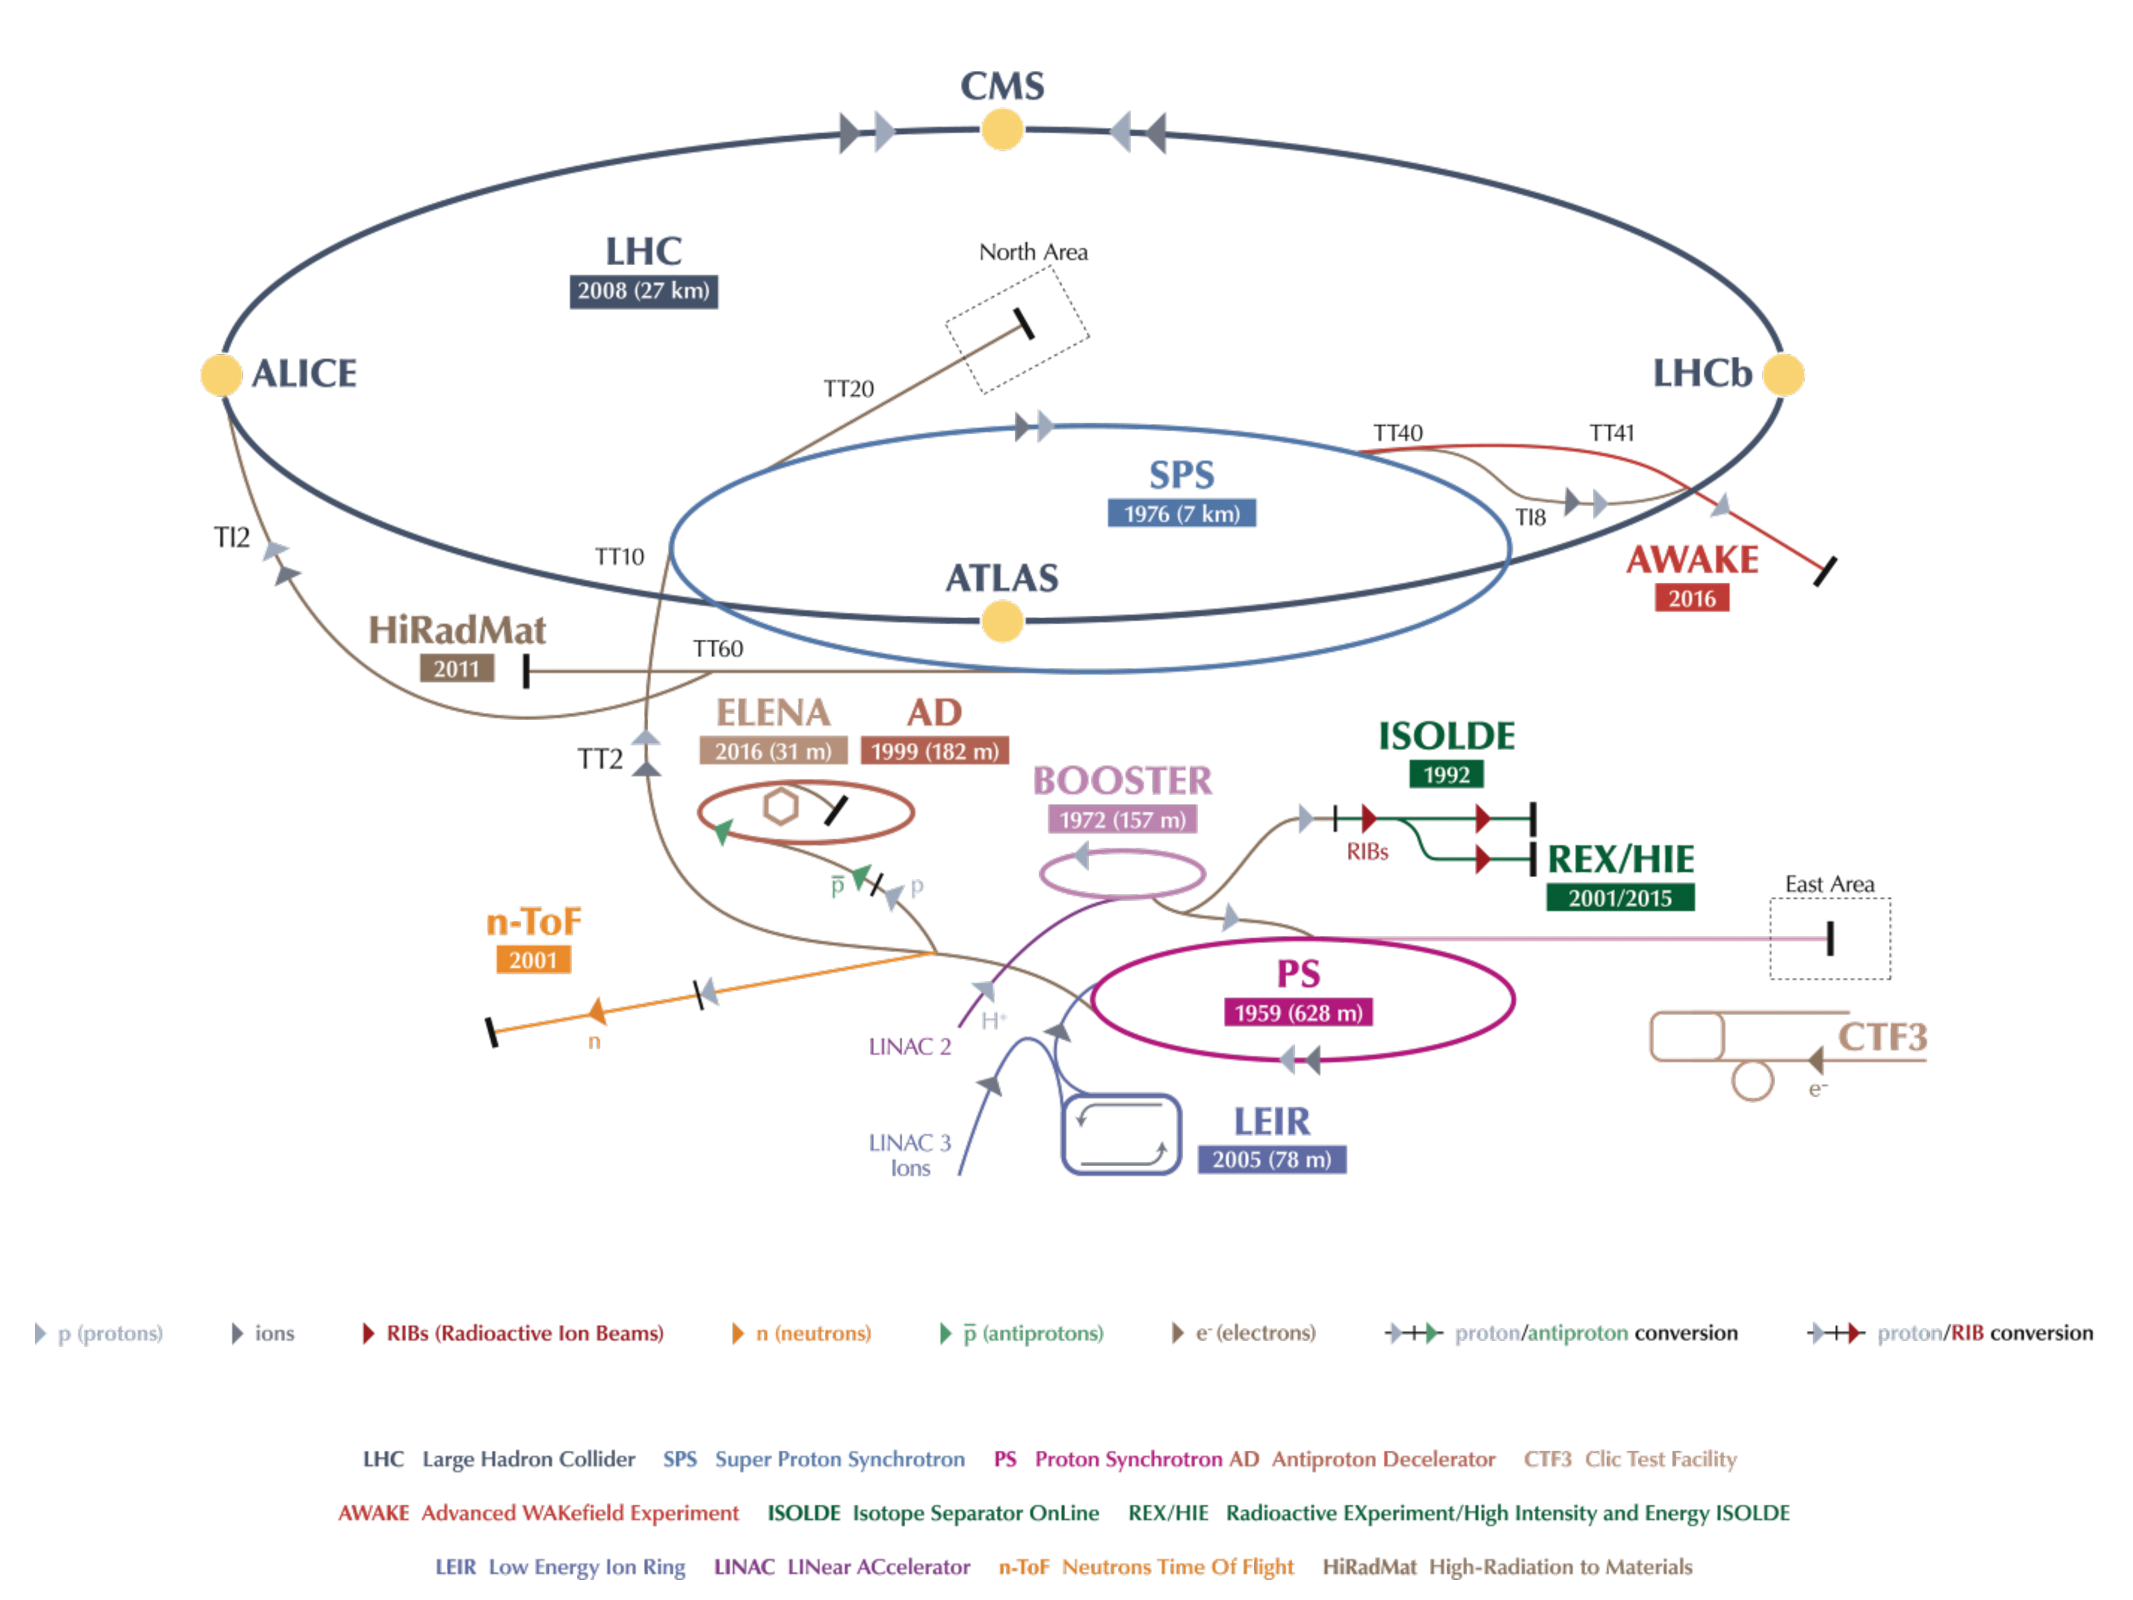
\includegraphics[width=0.72\linewidth]{figures/lhc_lhc.pdf}
\caption{CERN accelerator complex including the four main experiments and the injection chain}
\label{fig:lhc_lhc}
\end{center}
\end{figure}

\vspace{0.3cm}
Inside LHC particle collisions can happen at 4 interaction points of the tunnel, which correspond to 4 experiments: CMS, ALICE, ATLAS and LHCb. The ALICE experiment is designed to study the quark-gluon plasma using data collected during the heavy ion operation on the LHC. These measurements are designed to draw conclusions about the initial state of the universe. LHCb focuses on precisely measuring B-meson decays and CP-violating processes. CMS and ATLAS are the two general purpose experiments at the LHC build for studying a broad range of physics processes. These studies include precision measurements of Standard Model processes and parameters, thereby deepening our knowledge and understanding of the Standard Model. In addition, major fields of study are searches for the Higgs bosons and study of their properties and searches for physics beyond the Standard Model.

\section{The Compact Muon Solenoid (CMS) Experiment}

\subsection{Tracker} 
\subsection{Calorimeters} 
\subsubsection{Electromagnetic Calorimeter} 
\subsubsection{Hadronic Calorimeter} 
\subsection{Muon Chambers} 
\subsection{Data Acquisition and Trigger System} 
